\documentclass{beamer}
\usetheme{default}
\definecolor{LiUblue}{RGB}{0,185,231}
\usecolortheme[named=LiUblue]{structure}
%\beamerdefaultoverlayspecification{<+->}
\title{Quantifying nitrogen oxides and ammonia via frequency modulation in gas sensors}
\subtitle{Master Thesis - Mid term seminar}
\author{Marcos F Mourão}
\date{March 25, 2021}
 
 
 \usepackage{chemformula}
 \usepackage{url}
\begin{document}
	\begin{frame}
		\titlepage
	\end{frame}

\begin{frame}
	\frametitle{Outline}
	\tableofcontents
\end{frame}


\section{Problem recap}
\begin{frame}
	\frametitle{Problem in a nutshell}
	\framesubtitle{Motivation}
	$\text{NO}_{\text{x}}$\footnote{Image source: \href{http://www.nbrienvis.nic.in/Database/1_2039.aspx}{ENVIS Centre on Plants and Pollution}}:
	\begin{figure}[!htb]
		\centering
		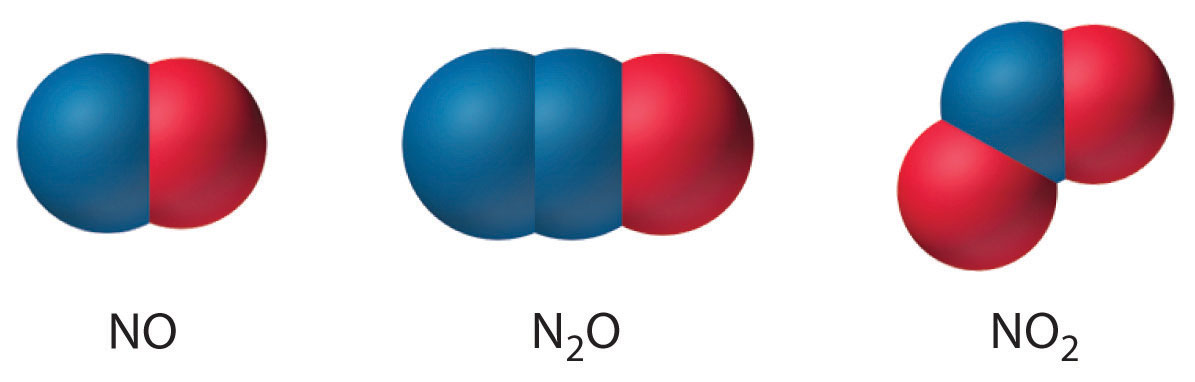
\includegraphics[width=0.6\textwidth]{../../figures/nox-molecules.jpg}
	\end{figure} 

	\pause
	\begin{itemize}
		\item NOx are detrimental to the environment and humans.
		\pause
		
		\item NOx are naturally ocurring in man-made processes. E.g. Combustion.
		\pause
		
		\item Ammonia can "neutralize" NOx, producing water (\ch{H2O}) and nitrogen gas (\ch{N2}). Both harmless! - Selective catalytic reduction (SCR).
		\pause
		
		\item But ammonia is also hazardous to the environment/humans.
	\end{itemize}
	
\end{frame}

\begin{frame}
	\frametitle{Problem in a nutshell}
	\framesubtitle{Motivation}
	
	\begin{itemize}
		\item The dosing of ammonia in the catalyst is key:
		\pause
		\begin{itemize}
			\item Too much ammonia: NOx reduction will occur $\rightarrow$ Unnecessary ammonia emissions.
			\pause
			\item Too little ammonia: NOx reduction will occur partially/will not occur $\rightarrow$ NOx emissions.
			\pause
		\end{itemize}
		\item Gas sensors can be used to measure the concentrations of NOx to aid on ammonia dosing.
		\pause
		\item However, the sensor also responds to ammonia.
		\pause
		\item Operating the sensor in a cyclic operation (e.g. temperature) can enhance selectivity.
		\pause
		\begin{itemize}
			\item Different gasses react differently in different stages of the cycle.
			\pause
		\end{itemize}
		\item Temperature cycling.
		\pause
		\item \textbf{Frequency cycling}.
	\end{itemize}
	
\end{frame}


\begin{frame}
	\frametitle{Problem in a nutshell}
	\framesubtitle{Research questions}
	\pause
	
	\begin{itemize}
		\item Can frequency cycling be used to simultaneously quantify NOx and ammonia concentrations?
		\pause
		\item Which method yield best prediction of gas concentrations?
	\end{itemize}
	
\end{frame}

\section{What has been done so far}
\begin{frame}
	\frametitle{What has been done so far}
	\pause
	\begin{itemize}
		\item Writing
		\pause
		\begin{itemize}
			\item Introduction - Done.
			\pause
			\item Theory - Partially done.
			\pause
			\item Data - Partially done.
			\pause
		\end{itemize}
		\item Some preliminary implementation of the methods
		\pause
		\begin{itemize}
			\item Linear Regression
			\pause
			\item Principal Component Regression
			\pause
			\item Partial Least Squares Regression
			\pause
			\item Ridge Regression
		\end{itemize}
	\end{itemize}
	
\end{frame}


\section{Caveats}
\begin{frame}

	\frametitle{Caveats}
	
	\begin{itemize}
		\item Real data not yet available - lab problems
		\pause
		\item Methods used on "dummy" data
		\pause
		\item Dummy data has problems:
		\pause
		\begin{itemize}
			\item Small number of observations
			\pause
			\item Measurement of shape features
			\pause
			\item Naïve window of measurements
			\pause
			\item High frequencies problematic
			\pause
		\end{itemize}
	\end{itemize}
	
\end{frame}

\section{(Dummy) data}
\begin{frame}
	
	\frametitle{(Dummy) data}
	\begin{figure}[!htb]
		\centering
		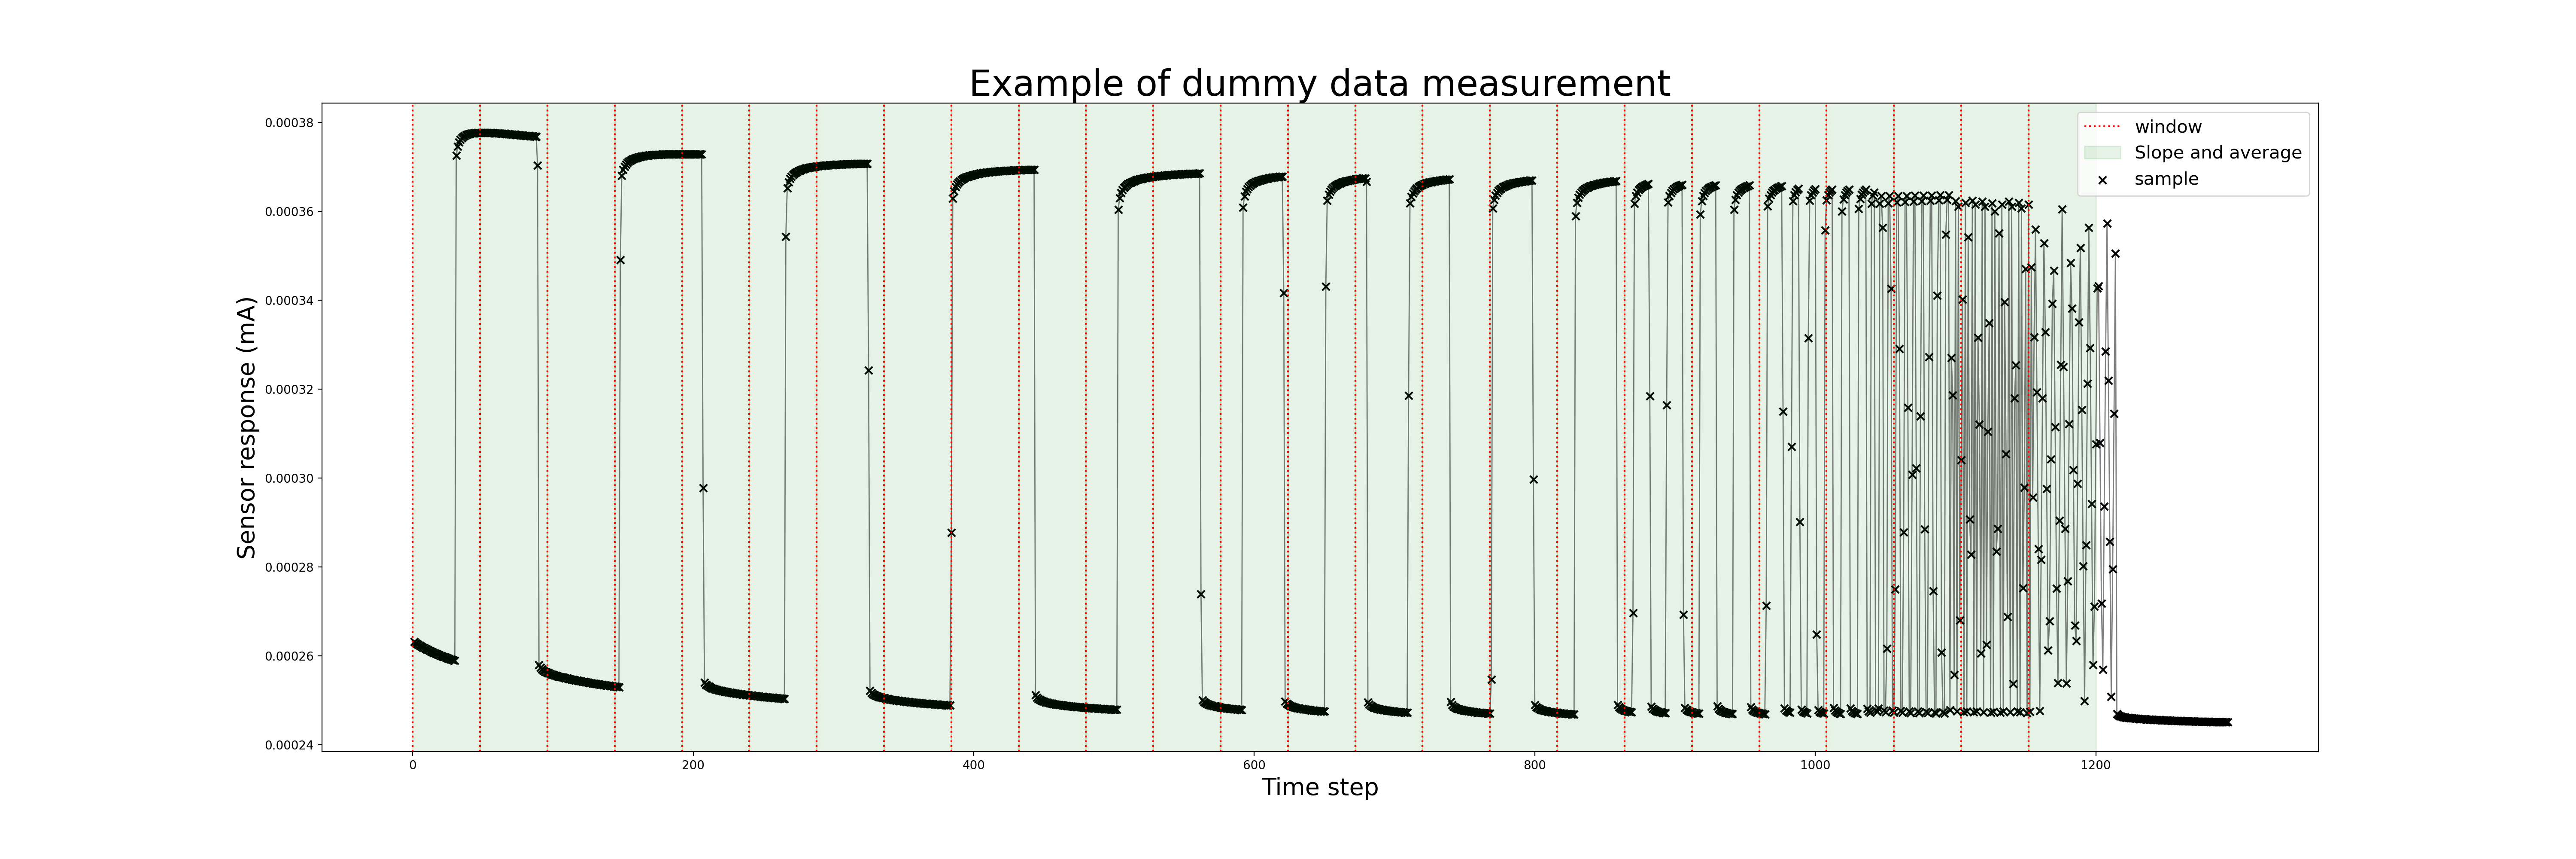
\includegraphics[width=1.2\textwidth]{../../figures/dummy-data.png}
	\end{figure} 

\end{frame}

\begin{frame}
	\frametitle{(Dummy) data}
	
	\begin{figure}[!htb]
		\centering
		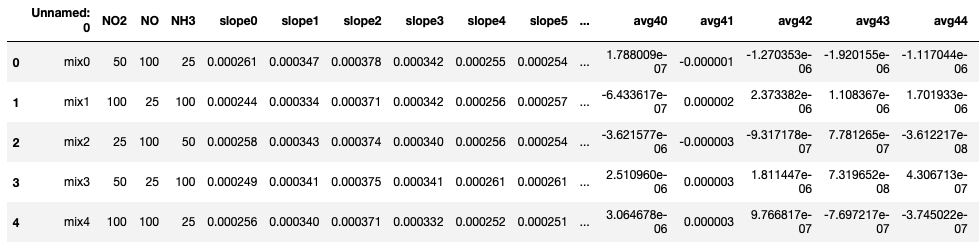
\includegraphics[width=1\textwidth]{../../figures/dummy-feats.png}
	\end{figure} 
	
 	\end{frame}


\section{Methods}
\begin{frame}
	
	\frametitle{Methods}
	\pause
	\begin{enumerate}
		\item Linear Regression
		\pause
		\item Principal Component Regression
		\pause
		\item Partial Least Squares Regression
		\pause
		\item Ridge Regression
		\pause
		\item Some non-parametric regression - tbd
	\end{enumerate}
	
\end{frame}


\section{(Preliminary) Results}
\begin{frame}
	\frametitle{(Preliminary) Results}
	\pause
	\begin{figure}[!htb]
		\centering
		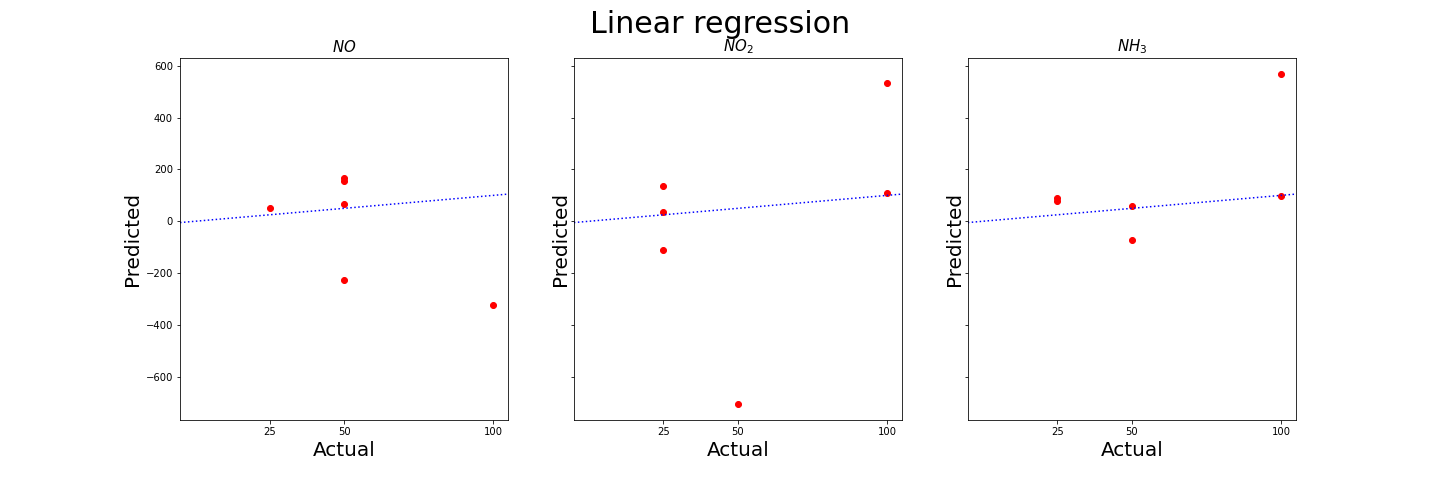
\includegraphics[width=1\textwidth]{../../figures/lr_plot.png}
	\end{figure} 
	\pause

\begin{figure}[!htb]
	\centering
	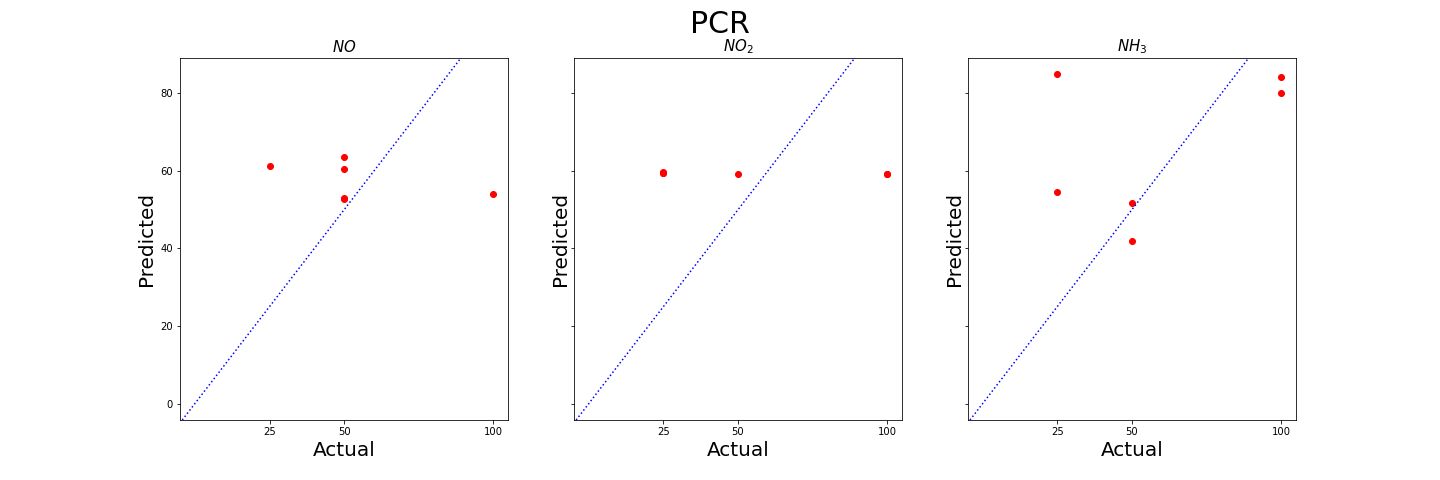
\includegraphics[width=1\textwidth]{../../figures/pcr_plot.png}
\end{figure}
\end{frame}

\begin{frame}
	\frametitle{(Preliminary) Results}
	\pause
	\begin{figure}[!htb]
		\centering
		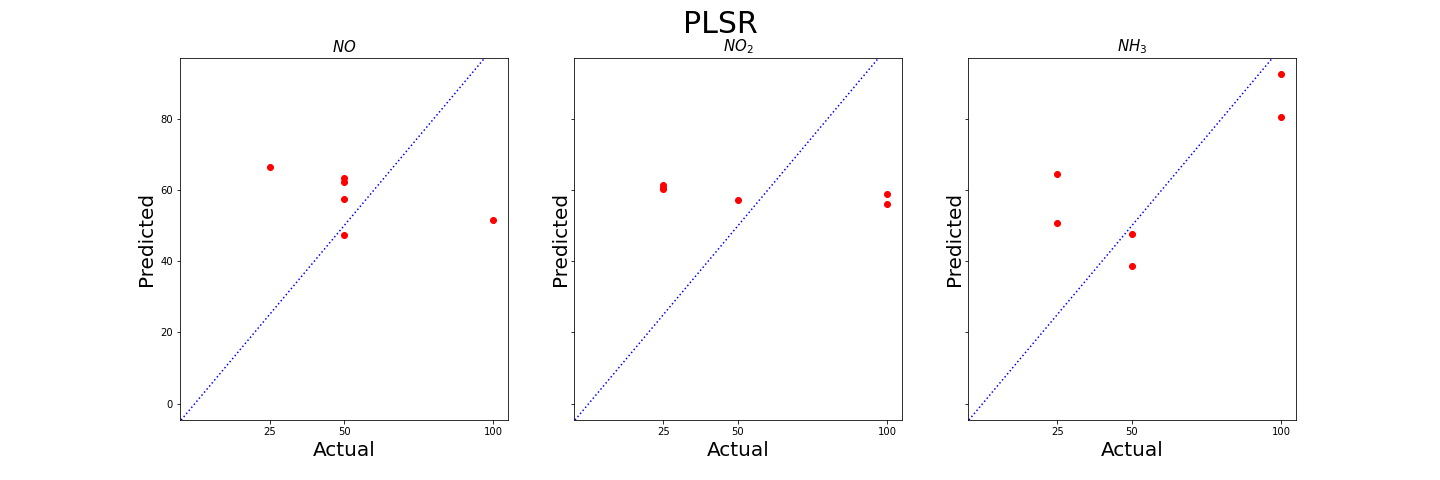
\includegraphics[width=1\textwidth]{../../figures/plsr_plot.png}
	\end{figure} 
	\pause
	
	\begin{figure}[!htb]
		\centering
		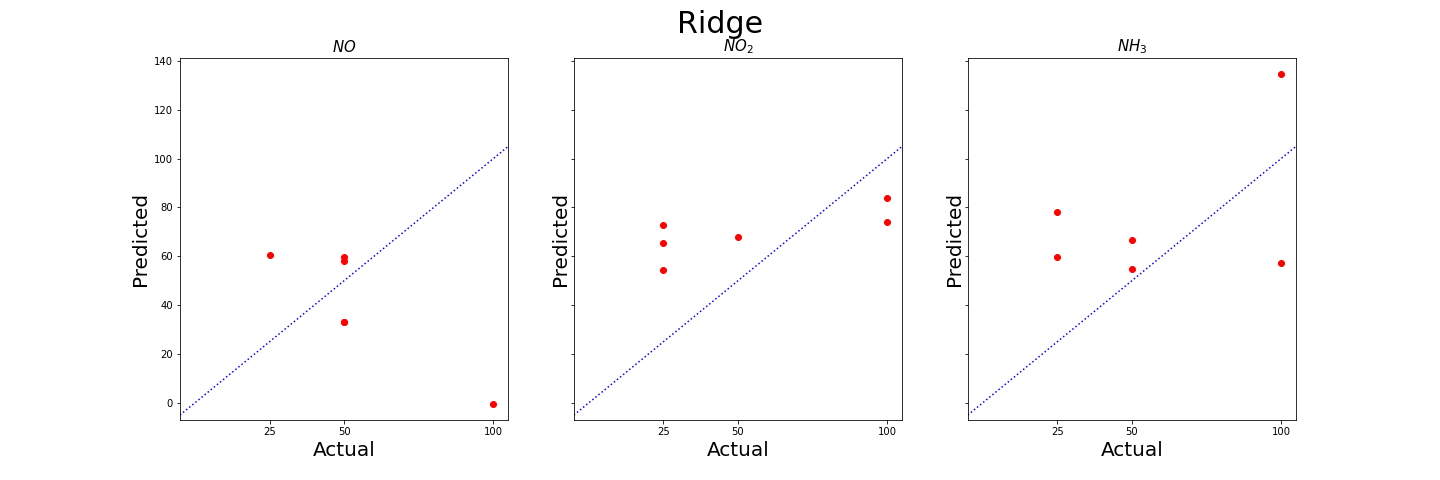
\includegraphics[width=1\textwidth]{../../figures/ridge_plot.png}
	\end{figure}
\end{frame}


\section{Real data}
\begin{frame}
	
	\frametitle{Real data will be much better!}
	\pause
	\begin{itemize}
		\item More gas mixtures
		\pause
		\item More frequencies
		\pause
		\item More cycles
		\pause
		\item Shape features directly measured
		\end{itemize}
\end{frame}

\begin{frame}
	\frametitle{Real data will be much better!}
	\pause
	\begin{table}[h]
		\centering
		\caption{Data acquisition details}
		\label{tab:measurements}
		\begin{tabular}{|c|c|}
			\hline
			\textbf{Parameter} & \textbf{Value} \\
			\hline
			Factors (gases) & 3 \\
			\hline
			Levels (concentrations) & 5 \\
			\hline
			Frequencies & 16 \\
			\hline
			Features per frequency & 4 (2 slopes and 2 averages) \\
			\hline
			Features per cycle & 64 \\
			\hline
			Number of cycles & 5 \\
			\hline
			Data points per mixture & 320 \\
			\hline
			Number of mixtures & 125 \\
			\hline
			Datapoints per experiment & 40.000 \\
			\hline
			Number of experiments & 3 \\
			\hline
			Total data points & 120.000 \\
			\hline
		\end{tabular}
	\end{table}
\end{frame}

\begin{frame}
	\frametitle{Real data will be much better!}
	\begin{figure}[!htb]
		\centering
		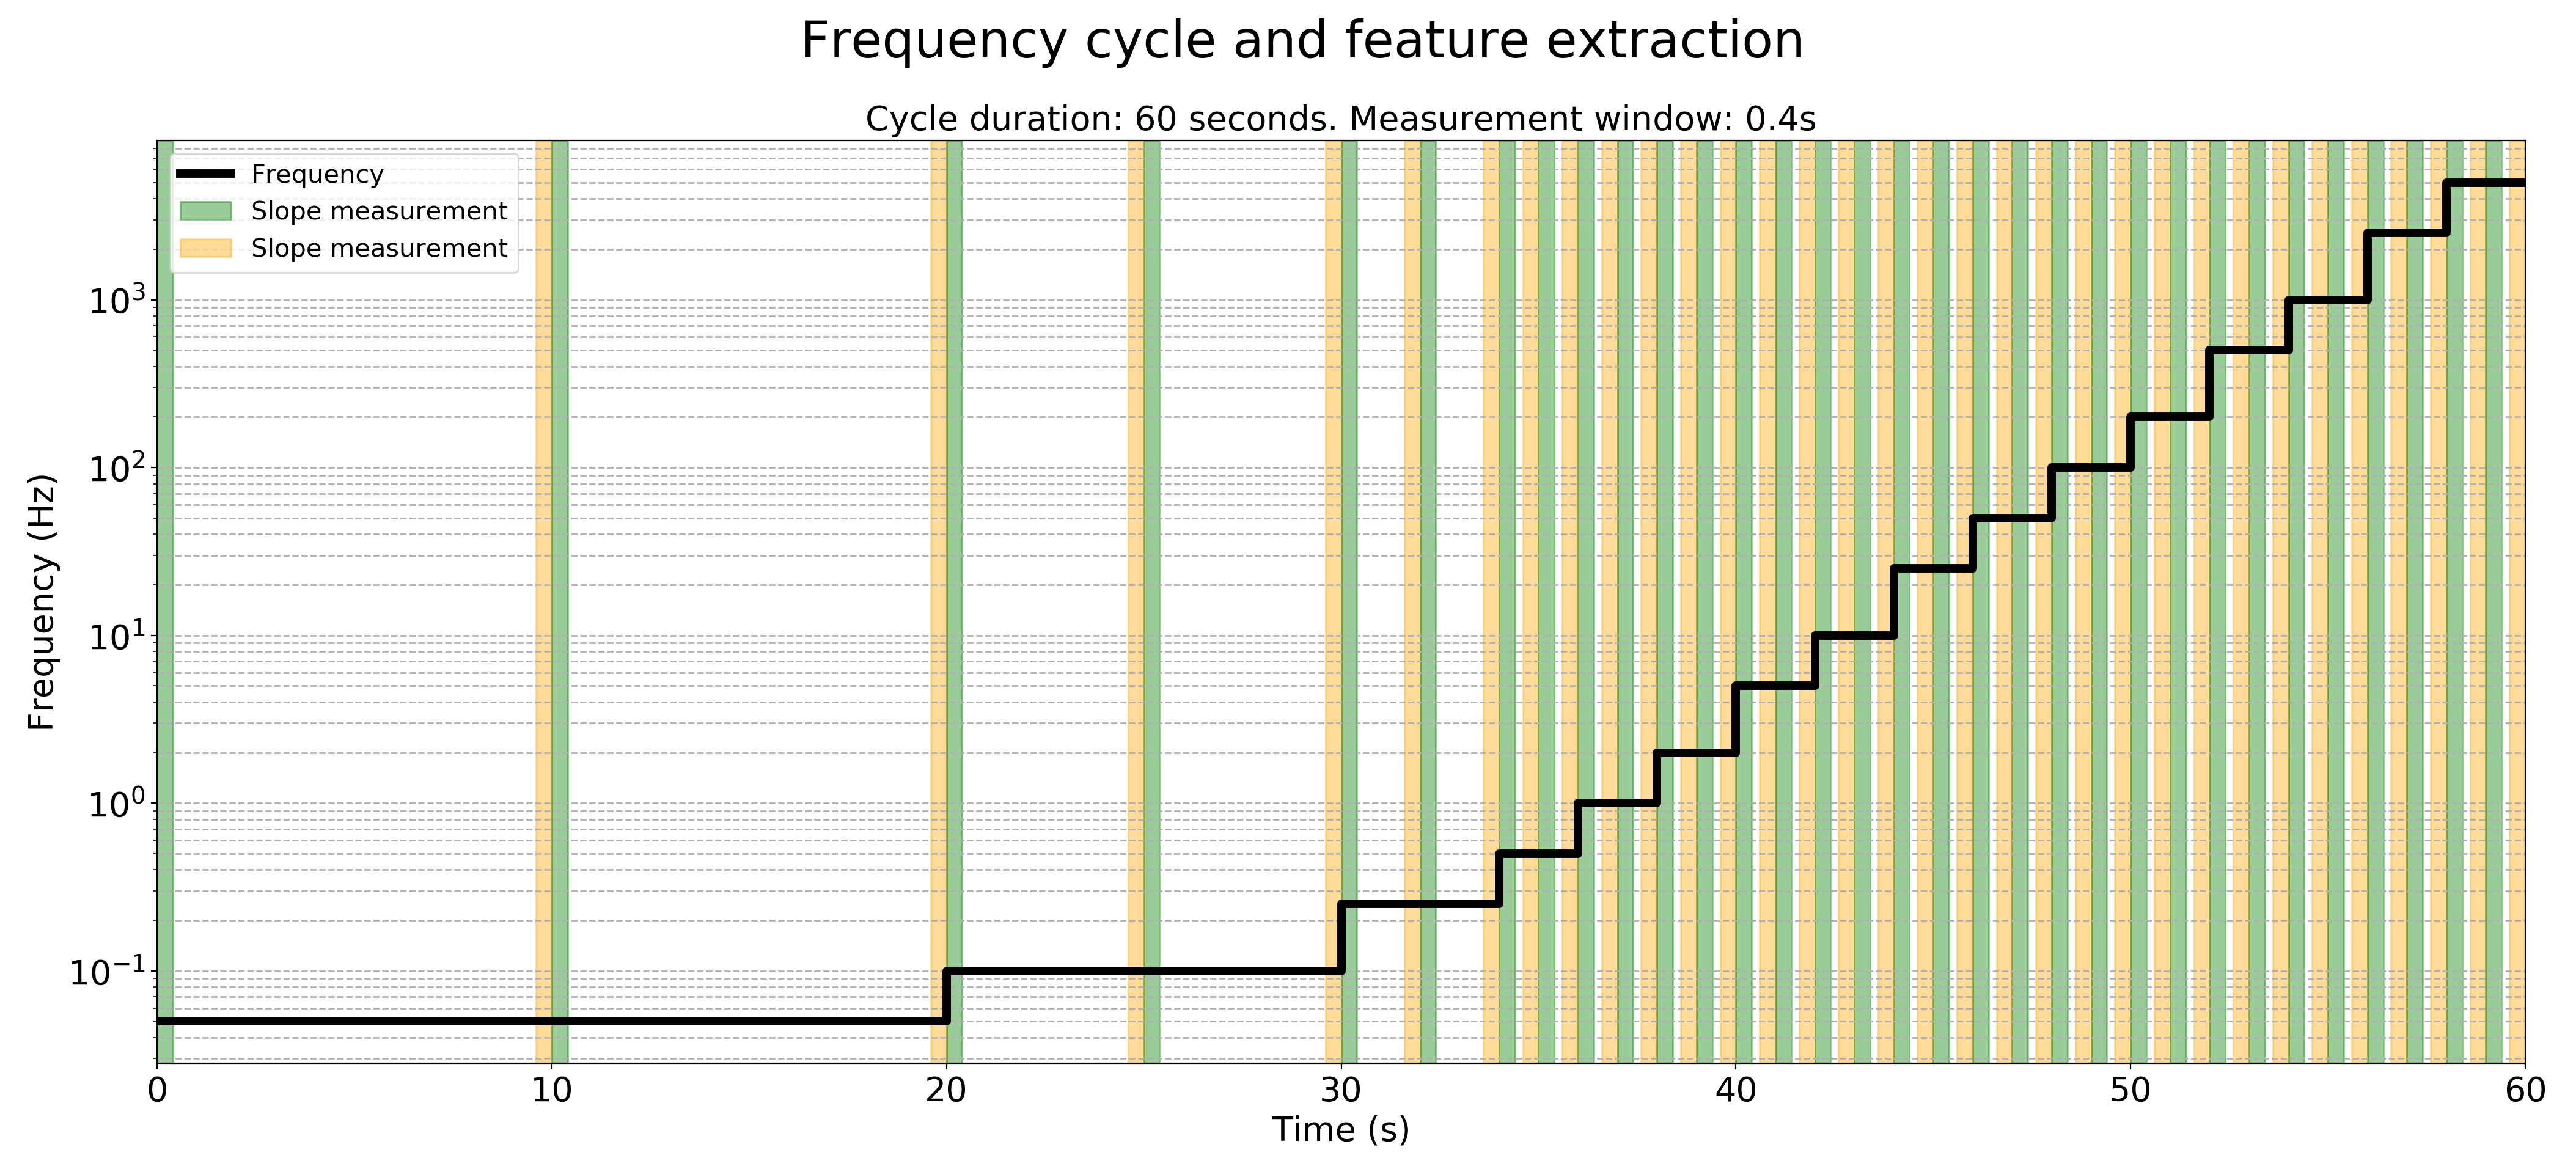
\includegraphics[width=1\textwidth]{../../figures/measurement-windows.png}
		\label{fig:feat-window}
	\end{figure} 
\end{frame}

\section{What is next}
\begin{frame}
	\frametitle{What is next}
	\pause
	\begin{enumerate}
		\item Apply methods to real data
		\pause
		\item Assess results
		\pause
		\item Define what is  "good" in "good prediction levels"
		\pause
		\item Look into non-parametric alternatives
		\pause
		\item Keep writing!
	\end{enumerate}
\end{frame}

\begin{frame}{}
	\centering \Huge
	\emph{Thank you!}
\end{frame}

\end{document}

